%-------------------------------------------------------------------
%-------------------------------------------------------------------
%----------------------   BA Andreas Korb   ------------------------
%-------------------------------------------------------------------
%-------------------------------------------------------------------


%%%%%%%%%%%%%%%%%%%%%%%%%%%%%%%%%%%%%
%%%%%%%%%%%%  Preamble  %%%%%%%%%%%%
%%%%%%%%%%%%%%%%%%%%%%%%%%%%%%%%%%%%%
\documentclass[
	11pt,			%Font size
	a4paper,		%Sheet size
	DIV=12,			%Type area (division into boxes)
	parskip=half,	%No indentation but line spacing for new paragraph
	headsepline,	%For dividing line on head side
	automark
	]{scrartcl}

%Todo Randausgleich

%Cross-platform
\usepackage[utf8]{inputenc}

%Font coding
\usepackage[T1]{fontenc}

%German Umlauts / Coding / Hyphenation
%\usepackage[ngerman]{babel}
%improved edge compensation
\usepackage{microtype}		

%Random text
\usepackage{blindtext}

\usepackage[hidelinks]{hyperref}

%Embed references
\usepackage{csquotes}
\usepackage{xcolor}
\definecolor{thi}{RGB}{0,90,155}
\hypersetup{
	colorlinks,
	linkcolor={thi},
	urlcolor={thi},
	citecolor={thi},
}

% sorting=none that they appear in the order they're used
\usepackage[sorting=none]{biblatex}

\addbibresource{references.bib}

%Set font
%Default cmr10 --> Computer Modern Roman 10pt (stored as bitmap)
\usepackage{lmodern}	%Vector version of cmr10

%\renewcommand{\familydefault}{\sfdefault}	%sf --> Without serifs

%Embed fonts
\usepackage{graphicx}
\usepackage{import}
\graphicspath{{images/}}

%Embed maths
\usepackage{amsmath,amssymb}

%Use euro sign
\usepackage[official]{eurosym}

%Improved table display
\usepackage{booktabs}

%Display table and figures next to text
\usepackage{wrapfig}


%%%%%%%%%%%%%%%%%%%%%%%%%%%%%%%%%%%%%
%%%%%%%%%%%%  Cover page  %%%%%%%%%%%
%%%%%%%%%%%%%%%%%%%%%%%%%%%%%%%%%%%%%
\author{Andreas Diemo Korb\vspace{9ex}}
\title{Evaluating approaches for more efficient UDS protocol scanning}
\subtitle{\vspace{1.5ex} to obtain the academic degree Bachelor of Science\vspace{3ex}}

\date{}

%Information on the bottom side of the cover sheet
\publishers{
	\begin{tabular}{rl}
		\textbf{Study program}	    & Bachelor Computer Science \\ 
		\textbf{Faculty}		    & Computer Science \\
		\textbf{Issue date}	        & \today \\
		\vspace{6ex}
	\end{tabular}
	
	\begin{tabular}{rl}
		\textbf{First supervisor}	& Prof. Dr. Hans-Michael Windisch \\
		\textbf{Second supervisor}	& Prof. Dr. Ulrich Margull \\
		\textbf{External supervisor}& Lukas Lisowski \\
		\textbf{External company}	& eMundo GmbH
	\end{tabular} 
}


%Header and footer
\usepackage[automark,footsepline,plainfootsepline]{scrlayer-scrpage}
\pagestyle{scrheadings}
\clearpairofpagestyles
\ihead{\leftmark}
\ifoot{Andreas Korb}
\ofoot*{\pagemark}

%THI Logo at the beginning of the cover page
\titlehead{
	\hfil	%Horizontal gap
	
\includegraphics[width=0.3\textwidth]{thi_logo_cropped}   \hspace*{3cm}
\includegraphics[width=0.3\textwidth]{emundo}
	\hfil
}


%%%%%%%%%%%%%%%%%%%%%%%%%%%%%%%%%%%%%%%%%
%%%%%%%%%%%%  Document begin  %%%%%%%%%%%
%%%%%%%%%%%%%%%%%%%%%%%%%%%%%%%%%%%%%%%%%
\begin{document}

\maketitle
\thispagestyle{empty}

\section*{Erklärung}
\thispagestyle{empty}
Hiermit erkläre ich, Andreas Korb, dass ich die vorliegende Seminararbeit zum Thema
\textit{Evaluating procedures for a more efficient information gathering with automotive diagnostic protocols.}
selbstständig angefertigt habe. Zudem habe ich diese nicht anderweitig für Prüfungszwecke
vorgelegt, keine anderen als die angegebenen Quellen oder Hilfsmittel benützt sowie wörtliche und sinngemäße Zitate als solche gekennzeichnet.
\vspace{3cm}

Ingolstadt, den 30.10.2020

\setcounter{tocdepth}{2} 	% Table of contents only Chapters and Sections
\thispagestyle{empty}
\tableofcontents



\setcounter{page}{0}
\section{Introduction}

\subsection{Motivation}
Nowadays a car is full of small computers handling tasks for the whole system. Without these helpers, functions like driver-assistance or self-diagnostic would not be possible. Those computers are generally called electronic control unit (ECU). Modern cars can contain over 100 of those. The complexity of ECU networks in a car is increasing quickly. The next generation of car networks is expected to be more centralized with less ECUs \cite{car-architecture}. This reduces complexity and its inherent risk of security vulnerabilities and high costs, as shown in \autoref{fig:centralized-architecture}.

%durations
\begin{figure}[h]
    \centering
    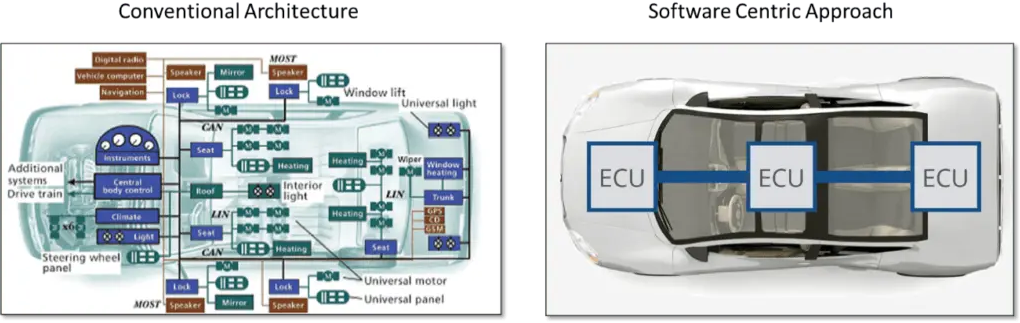
\includegraphics[width=1\textwidth]{centralized-architecture}
    \caption{Illustration of the current and the next-gen architecture of cars \cite{car-architecture}.}
    \label{fig:centralized-architecture}
\end{figure}

ECUs communicate with each other via bus systems. The most common ones are CAN, FlexRay and the Automotive Ethernet, which is becoming increasingly popular. Transport protocols usually sit on top of these physical layers. For Ethernet this is the well known TCP protocol, while the most common one for CAN is the ISO-TP protocol. Application protocols are used to ultimately transfer payload. For example, some protocols were created specifically for the development of units like Universal Measurement and Calibration Protocol (XCP) and some others were defined for diagnostic purposes such as Unified Diagnostic Services (UDS), General Motors Local Area Network (GMLAN) and On-board diagnostics (OBD). Both types are security critical. The XCP protocol is able to read and even write into the flash memory of an ECU. It shall be disabled on shipped ECUs. The UDS and GMLAN protocol provide definitions for diagnostic related tasks. However, diagnostic protocols are explicitly designed for actively used cars and thus exposed to the easily accessible OBD-II port, which by regulation must be present near the steering wheel on at least every car built after 2003 (see \autoref{fig:obd-port}). This fact makes them a great first target for gathering information. This work puts the UDS protocol in focus since it is the widest adopted protocol which allows extended functionality, for example flashing ECUs. The OBD protocol is excluded in this work because it does not offer any valuable information and the GMLAN protocol because it is restricted to vehicles from the General Motors corporation.

\begin{figure}[h]
    \centering
    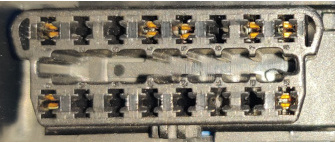
\includegraphics[width=0.5\textwidth]{obd-port}
    \caption{The OBD-II port of a BMW.}
    \label{fig:obd-port}
\end{figure}

The initial step in testing a system for weaknesses is to gather as much information from it as possible. In most cases, a protocol definition does not require that its specifications is fully supported; instead, a subset is sufficient.
Furthermore, a diagnostic protocol can define various states. The ECU may show varying behaviors in different states, for example support for other services. Since this kind of information is highly relevant for the security of the ECU, it would be helpful for security testers to gain this knowledge quickly and automatically.

One option to achieve this is to send all possible requests to an ECU and evaluate the responses. In the context of the project \emph{Penetration Test Driven Safety and Security System Improvements for Cyber-Critical Systems} (PetS3) \cite{pets3} such scanners have been implemented for UDS, GMLAN and OBD.

With their brute-force approaches, they are effective but not efficient. A scan can take a highly variable amount of time. It can range from a few hours to a day or more. In general, the more states are found on an ECU in a scan, the more time it will need. For example, more authentication information leads to more state detections and thus to higher runtimes. In addition, the response time of the ECU is also a decisive factor. The original runtimes observed of one UDS scan on the available ECUs are shown in \autoref{fig:durations} generated with the \mintinline{text}{plotly} library \cite{plotly}. It should be noted, that these scans have been executed with no additional information about the ECU as well. Accordingly, only the states that can be found without further information were detected.

%durations
\begin{figure}[h]
    \centering
    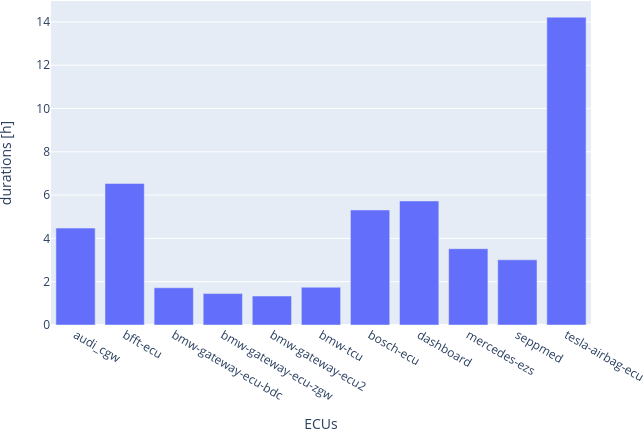
\includegraphics[width=1\textwidth]{durations}
    \caption{Observed runtimes for one UDS scan.}
    \label{fig:durations}
\end{figure}

Consequently, an efficient scan is desirable that keeps the scan time low even though many states can be found or the ECU has a high response time.

\subsection{Goal}

This paper evaluates different approaches to improve the efficiency of the UDS protocol scanning. The approaches can be mixed freely, if this leads to better results.

Efficiency improvement is understood as the ratio between the speed-up and the coverage. Coverage is here defined as the ratio of finds in the unmodified Scanner to the finds of the modified Scanner, and the speed-up as the saved time in comparison between these two. For both metrics, the higher the better.

Nevertheless, the coverage and speed-up have to be in balance. A speed-up of 90\% is not helpful if this results in 0\% coverage. The speed-up is achieved by reducing the number of generated packets. Hence, the challenge is to narrow down the scanning area to where positive responses are expected.


\subsection{Environment}
This work was created at eMundo GmbH in Ingolstadt. It is an IT service company which plans and executes projects for customers. Also, it is an aspiring company which in 20 years managed to open in total six company headquarters in Germany, Austria and Italy with almost 100 employees.

Since 2018, they are part of the \emph{Penetration Test Driven Safety and Security System Improvements for Cyber-Critical Systems} (PetS3) project. It is a collaboration research project among the OTH Regensburg, TH Nürnberg, EDAG Engineering Group AG, sepp.med GmbH, intive automotive GmbH and eMundo GmbH.

Due to the advancing networking, cyberattacks are a growing threat to a variety of application areas such as connected vehicles or smart metering. Common concepts of functional safety and IT security are required for these gateway-based systems. The aim of the research project is to investigate attacks on the IT security of system architectures of networked cyber-critical systems, since the interaction between functional safety and IT security is largely unknown in this context.

This paper is the final result of this project on the part of eMundo.

\subsection{Outline}

\section{Technical fundamentals}

This section will explain the technical fundamentals which are necessary to understand the full bachelor thesis.

\subsection{The Scapy library}
\label{sec:scapy}

%UDS stack
\begin{wrapfigure}{r}{0.15\textwidth}
    %
\includegraphics[width=0.1\textwidth]{scapy_logo}
    \raisebox{0pt}[\dimexpr\height-1.5\baselineskip\relax]{
\includegraphics[width=0.15\textwidth]{scapy_logo}}
    %\label{fig:scapy-logo}
\end{wrapfigure}

Scapy is a powerful interactive packet manipulation program. It is able to forge or decode packets of a wide number of protocols, send them on the wire, capture them, match requests and replies, and much more \cite{scapy}.

It is used through a text-based user interface. This has the advantage of being very lightweight, and working via ssh connections out-of-the-box. While being mainly a program, it can also be used as a library by importing the necessary classes and interfaces into the own Python program. Scapy supports Python 3 and additionally Python 2, even though its support has ended on 1st of January 2020. The following quote from a maintainer explains the reason behind that \cite{scapy-py2}:

\begin{displayquote}
    Scapy is a tool that can be used in a very large number of situations. Often, you don't get to choose the Python interpreter you have when you run Scapy. So, [...] we need to keep supporting Python 2.7 as long as we can.
\end{displayquote}

Understanding Scapy will be important for the later implementation in this work, since the UDS Scanner to be modified is built within Scapy.

One of the core classes in Scapy is the \textbf{Packet} class. All definitions of network packet layers, such as Ethernet, IP, TCP, CAN, UDS and so on, are defined in a class inheriting from that class.

The well-known and simple UDP protocol \cite{rfc768} serves as an illustrative example. It will be shown how the UDP header, shown in \autoref{fig:uds_header}, is translated to such a Scapy class.

%UDP header
\begin{figure}[h]
    \centering
    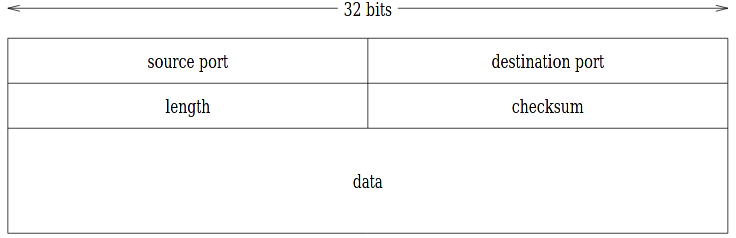
\includegraphics[width=0.7\textwidth]{udp_header}
    \caption{UDP header format \cite{udp_header}}
    \label{fig:uds_header}
\end{figure}

The UDP header format contains four fields and the data field. These four fields are translated literally into the Scapy class \textbf{UDP}. The data field is not part of it because Scapy uses an explicit operator to append data to the header information. This is shown later.

The following code snippet shows the mentioned class in the Scapy library.

\begin{samepage}
\begin{minted}{python}
class UDP(Packet):
   fields_desc = [ShortEnumField('sport', 53, UDP_SERVICES),
                  ShortEnumField('dport', 53, UDP_SERVICES),
                  ShortField('len', None),
                  XShortField('chksum', None)]
\end{minted}
\end{samepage}

As in common programmer language, \textbf{short} specifies 16 bits. Since the UDP header only contains 16 bits fields, the Scapy definition only includes \textbf{short} fields. The first parameter of a field is always the name of this field. \textbf{sport} stands for source port, and \textbf{dport} for destination port.
The next parameter sets the default value for this field. This is defined by the Scapy programmers to the best of their knowledge and not by the official UDP standard. \textbf{53} specifies the DNS protocol.
\textbf{EnumField}s also contain a third argument, a simple dictionary mapping from machine-readable values to human-readable texts. For example, part of the \textbf{UDP\_SERVICES} dictionary is: \mintinline{python}{{53: 'domain', 80: 'www_http'}}.
The difference between ShortField and XShortField is only the representation. The value of the XShortField will be displayed as a hex value and the ShortField as a decimal value.

The following snippet shows some examples of how to instantiate an object of the UDP class and also demonstrates how to append data to the headers with the “/” operator.

\begin{samepage}
\begin{minted}{python}
packet = UDP(dport=80) # is equivalent to:
packet = UDP(dport='www_http')

# Append 0x00 as data
packet = UDP(dport=80) / Raw(b'\x00')
\end{minted}
\end{samepage}

Now it shall be explained, how to actually send a packet and receive a response. For this, a socket is required. Scapy provides many kinds of sockets for different use cases. For example the \textbf{L2Socket} and the \textbf{L3PacketSocket}. The difference between them is that L2Socket expects a packet object containing all information starting from Ethernet (Layer 2), while L3PacketSocket expected a packet object only containing all information starting from IP (layer 3). The following code snippet uses the L2Socket for full coverage of the whole packet stack and explains how sending and receiving of a packet works (Note: Root privileges might be necessary for this to work):

\begin{samepage}
\begin{minted}{python}
# import necessary classes
from scapy.arch.linux import L2Socket
# Create a layer 2 socket specifing the interface name
socket = L2Socket('eth0')
# Create a packet covering layer 2 to 7, targeting the Google server
# This packet starts a TCP handshake, thus the SYN flag is exclusively set
# Set destination port to HTTP and a high source port
packet = Ether() / IP(dst='142.250.185.163') / TCP(flags='S', dport=80, sport=60123)
# sr1 stands for: send receive one
# it sends the given packet and returns the response
response = socket.sr1(packet)
# This displays the response in a human-friendly form
response.show()
\end{minted}
\end{samepage}

The .show() command gives the following output. It has been slightly edited to be more compact and some information has been replaced by placeholders for privacy reasons.

\begin{samepage}
\begin{minted}{text}
###[ Ethernet ]### 
  dst       = 12:34:45:67:89:ab
  src       = 2c:3a:fd:af:64:e0
  type      = IPv4
###[ IP ]### 
     version   = 4
     src       = 142.250.185.163
     dst       = 123.123.123.123
###[ TCP ]### 
        sport     = www_http
        dport     = 60123
        flags     = SA
\end{minted}
\end{samepage}

The SYN and ACK flags are now set as expected for the TCP handshake. Furthermore, the sport of the request is the dport of the response.


\subsection{The CAN bus}

All communication performed and recorded in this paper with an ECU is done via the Control Area Network bus.

\subsubsection{Basic information}

 Its specification is released in the ISO 11898. One packet on this bus can only transmit 8 bytes of payload.
 Each CAN packet has an identifier which a length of either 11 or 29-bits, the former being more common. An identifier does not necessarily have to designate a physical device; it can also specify one of several modules in that device.
 The maximum data rate is 1 Mbit/sec with a network length below 40 m. The higher the length, the lower the possible data rate, as can be seen in \autoref{tab:can-speed}.

\begin{table}[h]
    \centering
    \begin{tabular}{|c|c|c|}
    \hline
    \textbf{Bus Length (m)} & \textbf{Signaling Rate (Mbps)}\\
    \hline
    40 & 1 \\
    \hline
    100 & 0.5 \\
    \hline
    200 & 0.25 \\
    \hline
    500 & 0.10 \\
    \hline
    1000 & 0.05 \\
    \hline
\end{tabular}
\caption{Suggested Cable Length vs Signaling Rate \cite{slla270}.}
\label{tab:can-speed}
\end{table}

\subsubsection{Advantages}

This bus is robust because it is half-duplex, but still using two wires for the communication with differential signals. This means that if one wire is driven high, the other one is driven low. Thus, the receiver can reliably detect interferences by comparing these signals.

Moreover, CAN busses are using the bus network topology. This results in a smaller number of wires compared to star topologies, resulting in lower weight, which is an important factor for manufacturers (see \autoref{fig:with-without-can}).

%with-without-can
\begin{figure}[h]
    \centering
    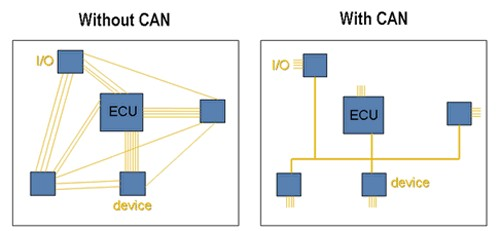
\includegraphics[width=0.7\textwidth]{with-without-can}
    \caption{CAN effect on decreasing the wire quantity \cite{Sharma2016}.}
    \label{fig:with-without-can}
\end{figure}

Last but not least, an important feature for the automotive application domain is the priority support. The lower the identifier, the higher the priority. Hence, if ECU1 and ECU2 transmit a CAN packet at exactly the same time, the packet with the lower identifier wins, the other one is discarded and will be retransmitted. This is called the Carrier Sense Multiple Access with Collision Detection (CSMA/CD) protocol \cite{Sharma2016}.

\subsubsection{Security vulnerabilities}

Thinking this one step further, CAN is vulnerable to denial of service attacks. This attack can be performed by flooding the CAN bus with zero-identifier messages resulting in drops of legitimate packets \cite{Buttigieg2017}.

Furthermore, Buttigieg et al. \cite{Buttigieg2017} describe three more security issues of the CAN bus protocol in their paper {Security Issues in Controller Area Networks in Automobiles}.
First, CAN packets do not contain any authentication information. An ECU receiving a message is not able to distinguish between a message from a legitimate ECU and a malicious one \cite{Buttigieg2017}. So, for example, if an ECUs state is changed to a higher privileged state, all devices, including malicious ones, will have access to its newly unlocked services. Countermeasures exist in the form of performing authentication, but there is no satisfying solution yet, which fulfills cost-effectiveness, backward compatibility, support for vehicle repair and maintenance, sufficient implementation details, and acceptable overhead \cite{Bozdal2020}.
Also, originally, CAN bus networks lacked network segmentation, since each message is broadcasted and received by each node of the network \cite{Buttigieg2017}. Nowadays, car networks of higher-class cars like Audi and BMW are usually divided into less and more critical segments by so-called Gateway ECUs \cite{Bozdal2020}. Despite the increase in the level of security, this makes it more difficult to maintain the system, which is associated with increased costs \cite{Bozdal2020}.
The final security vulnerability is the lack of data encryption \cite{Buttigieg2017}. Lightweight encryption systems could be implemented, but are limited by the short length of the data field (8 bytes) and the limited computing power of the ECUs \cite{Bozdal2020}.

Since all countermeasures described in the previous paragraph are limited, Intrusion Detection Systems (IDS) are emerging, with the advantages of not having to change the current CAN controller and not increasing bus traffic \cite{Bozdal2020}. Such a system has been implemented in the context of the PetS3 project \cite{spahn2018}.

\subsubsection{How to work with the CAN bus}

CAN interfaces are quite expensive, to communicate with ECUs paper the PCAN-USB from PEAK System was used in this work which costs by time of writing 180€. Instead, a virtual CAN interface can be used for simulations or simple tests. This is supported natively by Linux without additional actions.
To create a virtual CAN interface, only one command in a Linux shell is required:
\begin{samepage}
\begin{minted}{text}
sudo ip link add vcan0 type vcan
\end{minted}
\end{samepage}

The most common tool set to work with the CAN bus are the can-utils \cite{can-utils}, which can be usually installed with the package manager of the distributions. For example, the following command displays all messages of the CAN bus on interface \emph{vcan0}:
\begin{samepage}
\begin{minted}{text}
candump vcan0
\end{minted}
\end{samepage}

Another important task is to send a packet, which can be done with:
\begin{samepage}
\begin{minted}{text}
cansend vcan0 123#01.02
\end{minted}
\end{samepage}

This sends a CAN packet with the identifier 0x123 and the payload \emph{01 02}.

Alternatively, Scapy can be used. There are two implementations of CAN sockets, namely a native one, which uses the native Linux kernel module, and a software-based one, which uses the Python-CAN package.  The native implementation is only usable for Linux but the preferred one because it uses the socket interface of Linux and brings all its advantages, such as waiting for answers asynchronously while the own process doesn't require any CPU time. Python-CAN has the advantage of also working on Windows and macOS.

An equivalent Scapy script which accomplishes the same as the just described \mintinline{text}{cansend} command, is:

\begin{samepage}
\begin{minted}{python}
from scapy.contrib.cansocket_native import CANSocket
from scapy.layers.can import CAN
socket = CANSocket("vcan0")
socket.send(CAN(identifier=0x123, data=b"\x01\x02"))
\end{minted}
\end{samepage}

\subsection{The ISO-TP transport protocol for CAN}

CAN packets have a payload size of 8 bytes. This is sufficient for most UDS requests, but not for many UDS responses. Thus, ISO-TP is used as the transport protocol on the CAN bus for UDS communication.

\subsubsection{Basic information}

It is defined in ISO 15765-2 and increases the payload size from 8 bytes to 4095 bytes per message. At least one byte of each CAN packet is then transport protocol information, indicating whether this packet is a single frame or if it only contains a fragment of the actual payload.

\subsubsection{How to work with the ISO-TP protocol}

The can-utils tools also contain applications to handle ISO-TP communication. Since this is never used in this work, but the Scapy implementation is, only the Scapy implementation is explained.

As for the CAN implementation, there are two ISO-TP socket implementations in Scapy. A software and a native implementation. Until including Linux kernel 5.9, the corresponding ISO-TP module for Linux had to be installed separately \cite{isotp-module}. Since Linux kernel 5.10, it is part of the Linux mainline kernel \cite{isotp-commit}. Both implementations handle the ISO-TP metadata themselves, i.e.  fragmentation, defragmentation, etc.

An ISO-TP socket contains a source and destination identifier. They offer the same functionality as the ports for TCP or UDP. The source identifier is the identifier the outgoing CAN packets will contain. The destination identifier is the identifier expected for incoming packets.

The usage of the native implementation is illustrated in the following code snippet:

\begin{samepage}
\begin{minted}{python}
from scapy.contrib.isotp import ISOTPNativeSocket
socket = ISOTPNativeSocket('vcan0', sid=0x123, did=0x456)
packet = Raw(b'\x01\x02')
socket.send(packet)
\end{minted}
\end{samepage}

\subsection{The UDS protocol}

\subsubsection{Basic information}

UDS stands for \emph{Unified diagnostic services} and is an application protocol defined in ISO 14229 \cite{iso14229}. This protocol defines the structures of request and response packets for diagnostic purposes sent over an arbitrary data link.

%UDS stack
\begin{figure}[h]
    \centering
    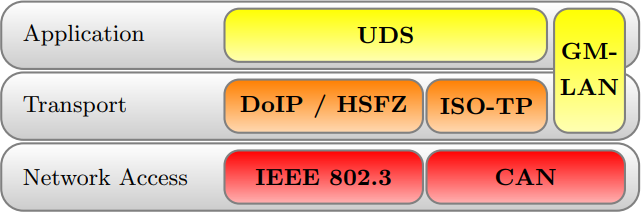
\includegraphics[width=0.7\textwidth]{uds-stack}
    \caption{The most common protocol stack for UDS \cite{Weiss2020}.}
    \label{fig:uds-stack}
\end{figure}

As shown in \autoref{fig:uds-stack}, the most common data links for the UDS protocol are the Ethernet and the CAN bus. Others can and are used as well, explicitly stated in the UDS standard are FlexRay, K-Line and LIN.

\subsubsection{Services}

The UDS protocol defines various services with different purposes. For example, the DiagnosticSessionControl service is used to enable different diagnostic states in the ECU. Its identifier is the number 0x10. All packets requesting this service specify this value as the first byte. The identifiers in the responses are defined as 0x40 added to the request identifier. Thus, for the DiagnosticSessionControl the positive response identifier is 0x10 + 0x40 = 0x50. A negative response always has the identifier 0x7f. This service is able to change the state of the ECU. Although the ReadDataByIdentifier service is not able to change the state, it is still very important. Data records in an ECU are stored with an identifier as the key. This service allows to read these values from an external device. Since there can be data stored, which is not meant to be read by everybody, there is another service called SecurityAccess, which allows to unlock these information for external devices. This mechanism is used for other services as well. The SecurityAccess service uses the challenge–response authentication in which an algorithm is the secret. It follows the following sequence \cite{iso14229}:

\begin{samepage}
\begin{enumerate}
  \item client requests the “Seed”,
  \item server sends the “Seed”,
  \item client sends the “Key” (appropriate for the Seed received),
  \item server responds that the “Key” was valid and that it will unlock itself.
\end{enumerate}
\end{samepage}

Now the implementation of UDS in Scapy is described.

\begin{samepage}
\begin{minted}{python}
class UDS(ISOTP):
    services = {
         0x10: 'DiagnosticSessionControl',
         # [...]
         0x22: 'ReadDataByIdentifier',
         # [...]
         0x7f: 'NegativeResponse'})
    fields_desc = [
        XByteEnumField('service', 0, services)
    ]
\end{minted}
\end{samepage}

%TODO: Why inherting from ISOTP

The UDS class contains only the service field. Even though the whole UDS protocol is in the application layer, the Scapy implementation starts a new class whenever the subsequent fields depend on one field of the current layer. This is the case here, since the next fields depend on the value of the service field. The service specific fields are defined in their own classes, for example:

\begin{samepage}
\begin{minted}{python}
class UDS_DSC(Packet):
    diagnosticSessionTypes = { ... }
    fields_desc = [
        ByteEnumField('diagnosticSessionType', 0,  diagnosticSessionTypes)
    ]
\end{minted}
\end{samepage}

A UDS packet enabling the extendedDiagnosticSession would be created with:

\begin{samepage}
\begin{minted}{python}
packet = UDS() / UDS_DSC(diagnosticSessionType='extendedDiagnosticSession')
\end{minted}
\end{samepage}

UDS not only allows to read data, but also to write. Which makes it especially critical for security. For example the firmware of an ECU can be updated through this protocol. This usually requires higher privileges, which can be gained through the previously mentioned SecurityAccess service.


\subsection{The UDS Scanner}

The UDS Scanner was implemented in Scapy for the PetS3 project.

\subsubsection{Purpose}

\begin{figure}[h]
    \centering
    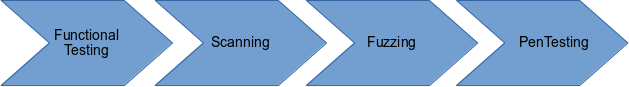
\includegraphics[width=0.8\textwidth]{automotive-security-testing-process}
    \caption{The Automotive Security Testing process.}
    \label{fig:automotive-security-testing-process}
\end{figure}

As \autoref{fig:automotive-security-testing-process} shows, the security testing process in the automotive domain consists of a scanning step \cite{Bayer2015}. This step aims detect which services of a protocol are implemented and what information can be retrieved there. The UDS Scanner fulfills these tasks. It can also be used for fuzzing and functional testing, even though scanning is its main use-case. The retrieved information assists for the manual PenTesting, the last step in this process.

\subsubsection{Enumerators}

% TODO: Add that it was still work in progress while doing this work
% and thus, that problems occured and had to be fixed.
% Out of scope of this work.

It executes so-called Enumerators which are service-specific and create all possible packets for a service.
For example, the enumerator for the DiagnosticSessionControl (DSC) service is called UDS\_DSCEnumerator. The most important member of the enumerator classes is the \mintinline{python}{_get_initial_requests} method. The return value is an iterable object which contains all requests for this service. DSC has an eight bit identifier, leading to a maximum of 2\textsuperscript{8} packets for this service. Each enumerator will be executed for each found state of the ECU. So, if an enumerator already ran, and afterwards a new state is found, this enumerator will run again within the same scan with the new-found state.

For a better understanding, the UDS\_DSCEnumerator implementation will be described exemplary.

\begin{samepage}
\begin{minted}{python}
class UDS_DSCEnumerator(UDS_Enumerator, StateGenerator):
    def _get_initial_requests(self, **kwargs):
        session_range = kwargs.pop('session_range', range(2, 0x100))
        return UDS() / UDS_DSC(diagnosticSessionType=session_range)
\end{minted}
\end{samepage}

The method can be given keyword parameters. The only one used here is \mintinline{python}{session_range}. If none is given, which is usually the case, it defaults to the range from 0x02 to 0xff. So, this enumerator creates 254 packets for each state. This service is a StateGenerator, which means its requests can change the state of the ECU. This is detected by the UDS Scanner and the new state will be scanned as well.

Special enumerators, called staged enumerators, can contain enumerators where each enumerator is a stage. They start scanning with the first stage for each state, followed by each subsequent stage in the same way. For each stage transition (for example $1 \rightarrow 2$ or $2 \rightarrow 3$) connectors can be defined. They are functions with two arguments, containing the previous enumerator and the new enumerator. Here the results of the previous enumerator can be evaluated and the new enumerator can be configured accordingly.

Enumerators can output their results as a text-table. For example:

\begin{samepage}
\begin{minted}{text}
---------------+---------------+---------------+---------------+
               | session1      | session1tp1   | session3tp1   | 
---------------+---------------+---------------+---------------+
TesterPresent: | PR: Supported | PR: Supported | PR: Supported | 
---------------+---------------+---------------+---------------+
\end{minted}
\end{samepage}

This means, the request of the TesterPresent service was positively answered by the ECU in all three found states. Session1 is the initial state the UDS Scanner starts with.

\section{Data gathering}
\label{sec:data-gathering}

From here, the procedure and the environment of gathering information to elaborate approaches will be discussed in detail.

\subsection{Test environment}

In order to find scan ranges that are likely to be answered positively, data from as many ECUs as possible is needed. In the context of the PetS3 project a remote testing environment has been created. This was particularly helpful in light of the contact limitations at the time of writing.

The infrastructure of Laboratory for Safe and Secure Systems (LaS3) was used for that. Specifically, their GitLab server was used, displayed in \autoref{fig:gitlab-screenshot}.

%GitLab screenshot
\begin{figure}[h]
    \centering
    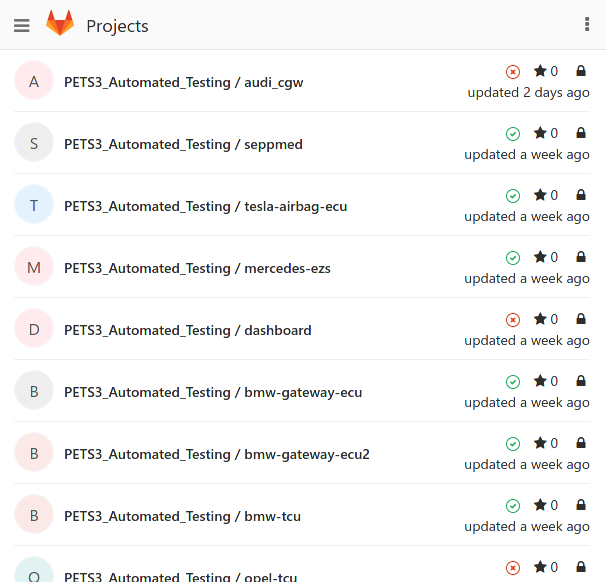
\includegraphics[width=0.7\textwidth]{gitlab-screenshot}
    \caption{Screenshot of the GitLab server.}
    \label{fig:gitlab-screenshot}
\end{figure}

Fourteen ECUs are available for testing on this server. Three of them are from Opel and thus only support GMLAN but not UDS.

For each ECU a YAML configuration file has been created. Various work is done here, for example installing this CAN-ISOTP module, if the running device is not at least on Linux 5.10 (see \autoref{sec:scapy}). Also, the current Scapy tree from the currently working branch is pulled and checked out.

Then, the actual tests are executed that are written in the pytest framework. Here, a UDS scan can be started. At the same time, another process is started to record all CAN traffic that takes place during the execution of the tests.

Finally, the resulting files are uploaded to the GitLab server so that they can be downloaded via a browser program.

\subsection{Explaining the stored data from one scan}

In total, five files are stored after a scan, which will be explained in this section.

\begin{itemize}
    \item candump.log
    \item generic.log
    \item profiling.csv
    \item milestones.csv
    \item data.pkl
\end{itemize}

The candump.log file is created by the candump program from the can-utils \cite{can-utils}. The generated files have a simple structure, each line representing one CAN packet.

\begin{samepage}
\begin{minted}{text}
(<timestamp>) <interface> <identifier>#<payload>
(1611779255.926425) can1 714#03225FB2CCCCCCCC
(1611779255.929936) can1 77E#037F2231AAAAAAAA
(1611779255.935338) can1 714#03225FB3CCCCCCCC
(1611779255.940680) can1 77E#037F2231AAAAAAAA
\end{minted}
\end{samepage}

Unfortunately, these resulting files contain a lot of information that is not only not needed, but also unwanted, as it leads to more difficult analysis and to higher storage usage. \autoref{fig:can-unwanted-information} shows the unnecessary information as it is ECU specific and does not add any value for the analysis.

%CAN unwanted information
\begin{figure}[h]
    \centering
    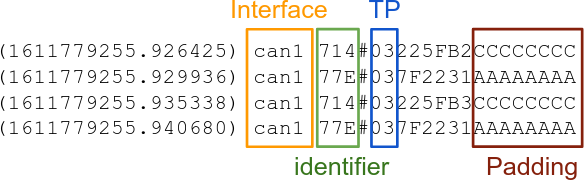
\includegraphics[width=0.7\textwidth]{can-unwanted-information}
    \caption{ECU specific information. TP = Transport protocol information}
    \label{fig:can-unwanted-information}
\end{figure}

Consequently, an abstraction is desirable. The newly created format is called the generic format. It removes the interface, the padding, resolves the transport protocol information (ISOTP) and replaced the identifier with mnemonics (s = Server, c = Client). Each line represents a full UDS packet, instead of a CAN packet as in the candump logs. \autoref{fig:candump-generic-conversion} illustrates the input and output of a conversion.

%candump to generic conversion
\begin{figure}[h]
    \centering
    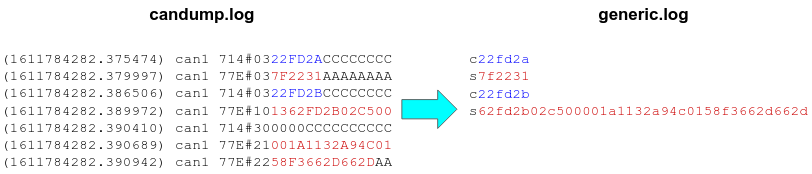
\includegraphics[width=1\textwidth]{candump-generic-conversion}
    \caption{candump.log to generic.log conversion.}
    \label{fig:candump-generic-conversion}
\end{figure}

This format proved to be very useful as it allows quick analysis by chaining common Linux programs.

For instance, counting the number of requests of one scan is a single command:
\begin{samepage}
    \begin{minted}{bash}
        $ grep '^c.*' -c generic.log
        988844
    \end{minted}
\end{samepage}

For profiling, two csv files have been added as output for the UDS scanner, namely profiling.csv and milestones.csv.

The former contains which enumerator ran under which state and when. It contains a fairly simple format, only containing the expected information:

\begin{samepage}
    \begin{minted}{text}
        state     ,enumerator       ,start            ,end
        ECU Reset ,ECU Reset        ,1611770228.135198,1611770228.658480
        [session1],UDS_CCEnumerator ,1611770228.661016,1611770231.236505
        ECU Reset ,ECU Reset        ,1611770231.236789,1611770231.754865
        [session1],UDS_DSCEnumerator,1611770231.756320,1611770231.895722
    \end{minted}
\end{samepage}

Each line in the milestones.csv contains a timestamp and the name of the final state of a found state path and its timestamp:

\begin{samepage}
    \begin{minted}{text}
        session1   ,1613302518.995168
        session2tp1,1613302569.605534
        session1tp1,1613309304.481464
        session3tp1,1613310988.231891
    \end{minted}
\end{samepage}

From this follows that a name can occur multiple times in this file, if there are more paths to the same state. What path will be taken is decided later in the UDS scanner after detecting it with the Dijkstra algorithm to find the shortest path.

Last but not least, the data.pkl file. Pickle is the object serialization module of the Python Standard library \cite{pickle}. The data.pkl file is the UDS scanner object after the scan, thus containing all results. This is helpful for debugging, analysis and also for simulation.

\subsection{Profiling the UDS Scanner}

The Pareto principle indicates that small number of causes can be responsible for a large percentage of effects \cite{pareto}. This is also applicable to optimization problems. Usually only a few number of code lines are responsible for the majority of the runtime. Optimizing them is far more effective than performing micro-optimizations as they naturally improve the performance to a great extent. Moreover, micro-optimizations are usually even more difficult to accomplish.

This is where the profiling.csv and the milestones.csv come into play to profile the UDS Scanner to find those places in need of optimization.

These files are used to create Gantt charts that show which parts of the UDS scanner take up most of its runtime. All diagrams in this work, including the Gantt charts, are generated with the library plotly for Python \cite{plotly}.

These Gantt charts have been created for each available ECU. For illustration one is sufficient since each chart showed the same gist (see \autoref{fig:tesla-gantt}).

\begin{figure}[h]
    \centering
    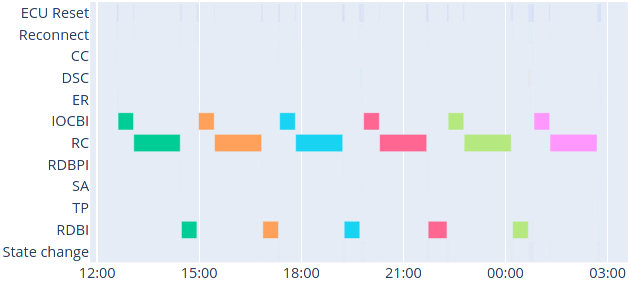
\includegraphics[width=1\textwidth]{tesla-gantt}
    \caption{Gantt chart of the Tesla-Airbag-ECU.}
    \label{fig:tesla-gantt}
\end{figure}

The time is represented on the x-axis and the enumerators and events are listed on the y-axis. One color represents one state of the ECU.
Although it seems that some enumerators and events do not require time, their time consumption is only so small that they are not or hardly visible in this scaled-down version of the diagram.

The main cause of runtime is the RCEnumerator. This was expected, since this is the enumerator with the most generated requests. In second place are the IOCBIEnumerator and the WDBISelectiveEnumerator. The latter consists of actually two enumerators, the RDBIEnumerator and the WDBIEnumerator. The RDBIEnumerator generates more requests than the WDBIEnumerator to a large extent, which accordingly hardly contributes to the runtime. Therefore, for simplicity, this enumerator will be called RDBIEnumerator from here on.
The IOCBIEnumerator and RDBIEnumerator generate about the same runtime, this was to be expected since they generate the same number of requests. The RDBI service is much more frequently supported by ECUs than the IOCBI service, resulting in a smaller database, so it was decided that the RDBI service would be optimized instead of the IOCBI service.

In summary, the RCEnumerator and the RDBIEnumerator are the most critical performance barriers of the UDS scanner and therefore belong to the subjects to optimize.

\include{chapters/4_profiling}
\section{Approaches}

This section discusses the optimization of the two enumerators from the previous section, each using a different approach. In addition, a third approach discussed is to avoid scanning unsupported services. 

\subsection{Use information of a former service scan}

This approach aims to reuse information from one enumerator in a later enumerator within the same scan. This will be applied to the RCEnumerator.

\subsubsection{Current behavior}

The Routine Control service is used by the client to execute a defined sequence of steps and obtain any relevant results \cite{iso14229}. For a quick overview of the service a simplified code snippet of the Scapy implementation is used.

\begin{samepage}
\begin{minted}{python}
class UDS_RC(Packet):
    routineControlTypes = {
        1: 'startRoutine',
        2: 'stopRoutine',
        3: 'requestResults'
    }
    fields_desc = [
        ByteEnumField('routineControlType', 0, routineControlTypes),
        XShortField('routineIdentifier', 0)
    ]
\end{minted}
\end{samepage}

The \mintinline{python}{routineControlType} field specifies what should happen to a routine. Possible are starting, stopping and requesting the results. To specify which routine is to be controlled, there is the \mintinline{python}{routineIdentifier} field. Hence, there are three control types, and because the identifier is a short field, there are 2\textsuperscript{16} identifiers. This leads to the following formula, showing how many requests are generated for a UDS scan:
\[f(n)=3 \cdot 2^{16} \cdot n\]
wherein $n$ stands for the number of detected states.

The current RCEnumerator does exactly this, it generates the full range for each state. That's what needs to be reduced. Its current behavior is illustrated in \autoref{fig:rc-behavior-current}. The green areas symbolize the scanned ranges.

\begin{figure}[h]
    \centering
    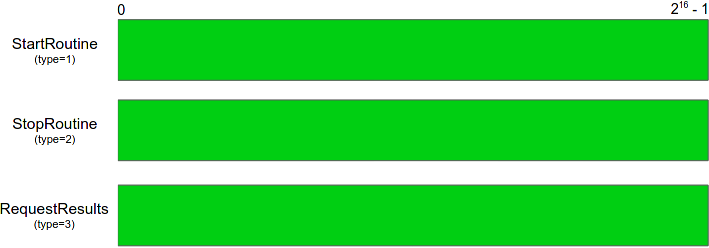
\includegraphics[width=0.8\textwidth]{rc-behavior-current}
    \caption{Current procedure for scanning the RC service.}
    \label{fig:rc-behavior-current}
\end{figure}

\subsubsection{Elaborating the new behavior}

As a first step to find a way to apply the approach to the RCEnumerator, the distribution of the identifiers is visualized grouped by the type as a histogram in \autoref{fig:rc-distribution}.

% TODO: maybe to attachments
\begin{figure}[h]
    \centering
    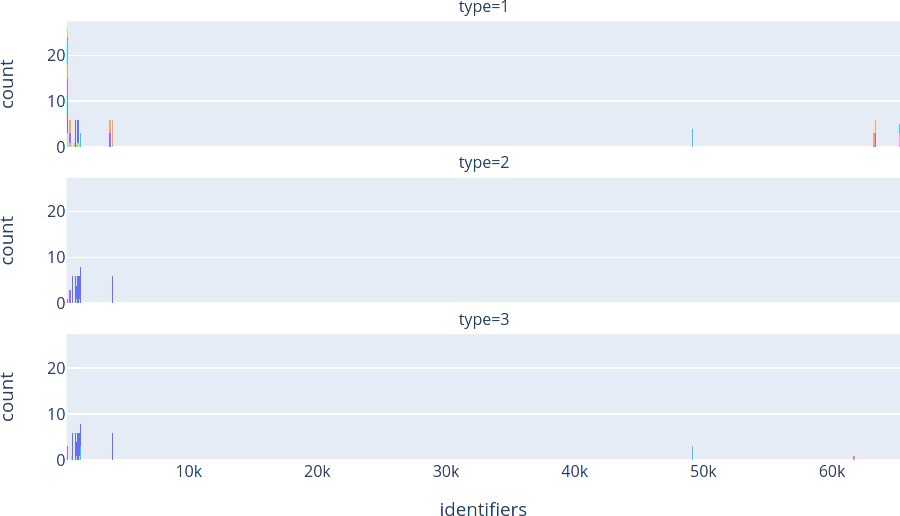
\includegraphics[width=0.8\textwidth]{rc-distribution}
    \caption{Distribution of the RC identifiers. Each color is one ECU.}
    \label{fig:rc-distribution}
\end{figure}

It can be seen that if an identifier is available in Type1, it is likely that this identifier also occurs in Type2. Consequently, if an identifier does not respond positively in Type1, it is also very unlikely that it will respond in Type2 or Type3. This appearance is used to reduce the scan range for this service.

The new behavior starts with scanning all 2\textsuperscript{16} identifiers with Type1. So, 2\textsuperscript{16} is the minimum number of requests for each state with the new behavior. Only the identifiers, which led to a positive response, are scanned with Type2 and Type3 as well. Moreover, it was observed that there seems to be a locality effect for the identifiers. Thus, if an identifier with Type1 is answered positively, scanning nearby identifiers instead of just that identifier will result in higher coverage. What needs to be found out is the block size which leads to the best coverage, while maintaining an appropriate speed-up. \autoref{fig:rc-behavior-new} illustrates that. The green areas again show the scanned ranges, additionally, the red areas are the found identifiers in Type1 and their resulting ranges for Type2 and Type3 and the gray areas show the areas that were not scanned and thus how much time was saved.

\begin{figure}[h]
    \centering
    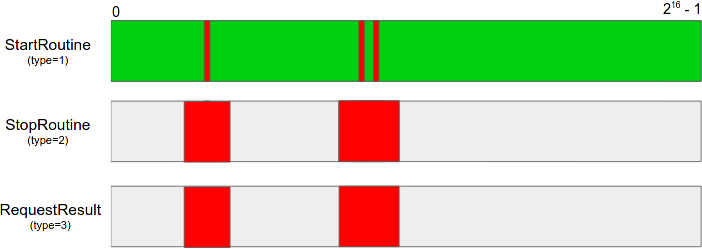
\includegraphics[width=0.8\textwidth]{rc-behavior-new}
    \caption{New procedure for scanning the RC service.}
    \label{fig:rc-behavior-new}
\end{figure}

The limits of the speed-up are defined as following:
\[ 0\ \% \ \leq\  s(n)\  \leq 66.\overline{6}\ \% \quad \forall \  n \in \left\{0, 1, ..., 2^{16} \cdot 3\right\} \]
%\[ 0\  \ \leq\  s(n)\  \leq \frac{2}{3} \quad \forall \  n \in \left\{0, 1, ..., 2^{16 * 3}\right\} \]
wherein $s$ is the speed-up function and $n$ the number of generated requests for this service.

The reason for the upper limit of $66.\overline{6}$ \% is that Type1, which is one third of all possible requests, is always scanned completely.

To find out the best value, scans with different block sizes are simulated. For a quick simulation another observation is used. If one identifier is available in one state, it is likely to be available in the other states too. Thus, the states are ignored in the simulation, which improves the performance by a multiple, while it is still very close to the real ECUs. The simulation only uses information gathered from the real ECUs as described in \autoref{sec:data-gathering}. Specifically, the required information is extracted from the generic.log file.

As described, the simulation starts with getting all identifiers which have been positively answered by the currently simulated ECU. Subsequently, these identifiers are expanded to both sites from 0 to 200. Overlapping blocks are resolved to one continuous space. With these blocks the coverage and the number of requests can be calculated. The number of requests can be converted to the speed-up. The results are averaged.
The blocks are expanded to both sites. So, for example, if the identifier 500 has been answered positively and the expansion size is 100, it leads to block from 400 to 600. A simulation was also run with expanding individual identifiers in to one site only, which yielded very similar results. Thus, it was left with the expansion in both directions. 
The following pseudocode shows the procedure more clearly.

\begin{samepage}
\begin{minted}{python}
coverages = []
speedups = []
for expansion_size in range(200):
    coverages_block = []
    speedups_block = []
    for ecu in ecus:
        ids_type1 = get_type1_ids(ecu)
        to_scan = ids_to_block(ids_type1, expansion_size)
        coverages_block.append(get_coverage(ecu, to_scan))
        count_requests = len(to_scan)
        speedups_block.append(get_speedup(ecu, count_requests))
    coverages.append(avg(coverages_block))
    speedups.append(avg(speedups_block))
\end{minted}
\end{samepage}

The results of this simulation are plotted in \autoref{fig:rc-simulation-result}. The speed-up is linear to the expansion size. That makes sense, because the larger the blocks are, the more requests are generated. The expansion size of zero represents the results without using the locality effect. The maximum difference in coverage between with and without locality effect are 22\%, even though the maximum speed-up difference is only 1\%.

\begin{figure}[h]
    \centering
    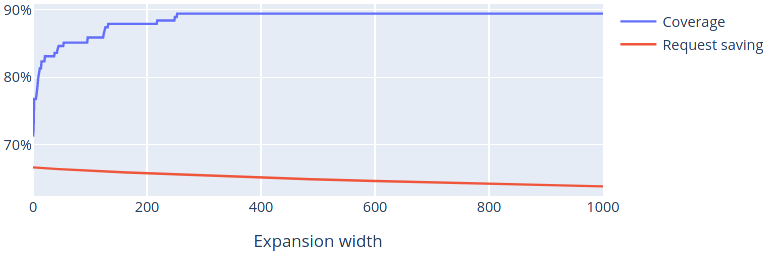
\includegraphics[width=0.7\textwidth]{rc-simulation-result}
    \caption{Simulation result for the RC enumerator.}
    \label{fig:rc-simulation-result}
\end{figure}

Since the speed-up is high for each simulated block size, the highest coverage was chosen which starts with block size \textbf{132}. Hence, this value is the chosen and implemented block size.

\subsubsection{Implementation}

Three classes are of interest:

\begin{itemize}
    \item \textbf{RCEnumerator}: Defaults to scanning the whole RC service, including all three types.
    \item \textbf{RCStartEnumerator}: Only scanning Type1 of the RC service.
    \item \textbf{RCSelectiveEnumerator}: Staged enumerator containing an RCStartEnumerator and an RCEnumerator.
\end{itemize}

\begin{figure}[h]
    \centering
    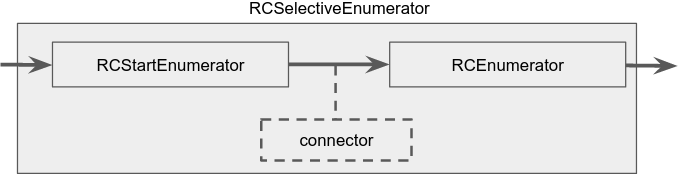
\includegraphics[width=0.7\textwidth]{rc-schematic}
    \caption{Schematic illustration of the new RCSelectiveEnumerator.}
    \label{fig:rc-schematic}
\end{figure}

The RCSelectiveEnumerator connects its two stages with a connector function that is called as soon as the first stage is done and the second is to be started. It expands the found identifiers of the RCStartEnumerator to ranges and also resolves any overlaps to a continuous range and forwards these ranges to the second stage, the RCEnumerator. Additionally, the connector configures the RCEnumerator to only scan Type2 and Type3.

Each positively answered identifier of Type1 in any state will also be probed for all subsequent states in Type2 and Type3, even if this identifier is not found in Type1 for another state. This increases the coverage in cases, where a routine can be started in a state, but its result, or to stop it, may only be requested in another state. It also hardly leads to more requests, which can be seen at the speed-ups in \autoref{fig:rc-schematic}.

\subsubsection{Evaluation}

\begin{table}[h]
    \begin{center}
    \begin{tabular}{ccc}
        \hline
        & \textbf{Coverage} & \textbf{Speed-up} \\
        \hline
        \textbf{audi\_cgw} & 87.6\% & 65.4\% \\
        \textbf{bfft-ecu} & 100\% & 66.2\% \\
        \textbf{bmw-gateway-ecu-bdc} & 100\% & 66.2\% \\
        \textbf{bmw-gateway-ecu-zgw} & 100\% & 64.5\% \\
        \textbf{bmw-gateway-ecu2} & 100\% & 64.6\% \\
        \textbf{bmw-tcu} & 100\% & 66.7\% \\
        \textbf{bosch-ecu} & 100\% & 64.6\% \\
        \textbf{dashboard} & 50.0\% & 66.2\% \\
        \textbf{mercedes-ezs} & 100\% & 65.1\% \\
        \textbf{seppmed} & 100\% & 66.2\% \\
        \textbf{tesla-airbag-ecu} & 100\% & 66.7\% \\
        \hline

    \end{tabular}
    \end{center}
    \caption{Measured coverages and speed-ups on ECUs with approach 1.}
    \label{tab:evaluation-approach1}
\end{table}

9 of 11 ECUs had a full coverage. The coverage for the dashboard ECU notable low. Therefore, a closer look was taken there again. It turned out that the Dashboard only supports two identifiers. The identifier 515 for Type1 and identifier 61,728 for Type3. The former is detected, but the resulting range for Type3 is far from the identifier 61,728. Hence, the loss and a coverage of 50\%.

The speed-up is calculated by comparing the number of requests sent with the selective enumerator and the number of requests that would have been sent with the old enumerator for an entire scan. For each ECU it is close to the theoretical maximum of $66.\overline{6}$ \%, leading to the evaluation that there is a great potential in this approach.

The use of information within the same scan is applicable to scans of services with multiple fields, as it is the case with the RC service that has the \mintinline{text}{routineControlType} and \mintinline{text}{routineIdentifier} fields. This results in a high scan time for this service and thus a high potential time savings. However, if an identifier is not recognized in the first scan, it will not be recognized in the next scans as well.


\subsection{Reduction of scan range}
Most services are simpler and don't have a type as the RC service but only an identifier. So, reusing information within the same scan is limited. Here the second approach will be applied to the Read Data By Identifier (RDBI) enumerator. The idea is to scan more heavily the blocks where positive behavior is more likely than others. The approach will be applied.

\subsubsection{Current behavior}

The Read Data By Identifier service allows the client to request data record values from the server identified by one or more dataIdentifiers \cite{iso14229}. Again, for a quick overview of the service a simplified code snippet of the Scapy implementation is used.

\begin{samepage}
\begin{minted}{python}
class UDS_RDBI(Packet):
    fields_desc = [
        XShortField('identifier', 0)
    ]
\end{minted}
\end{samepage}

To specify which data record to retrieve, there is the \mintinline{python}{identifier} field. Hence, because the identifier is a short field, there are 2\textsuperscript{16} identifiers. This leads to the following formula, showing how many requests are generated for a UDS scan:
\[f(n)=2^{16} \cdot n\]
wherein $n$ stands for the number of detected states. 

So, the current RDBIEnumerator is very simple. It generates 2\textsuperscript{16} packets counting up from 0 to 65535 and generating for each number a packet with this number as identifier for each state.

\subsubsection{Elaborating the new behavior}

As a first step, the distribution of identifiers over all ECUs is visualized in a histogram to check if there is potential. The result can be seen in \autoref{fig:rdbi-distribution}.

\begin{figure}[h]
    \centering
    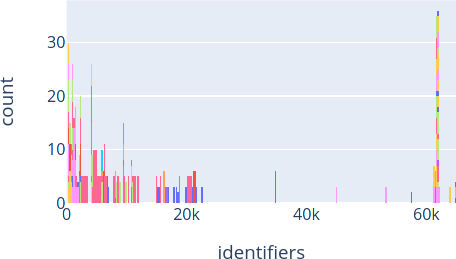
\includegraphics[width=0.7\textwidth]{rdbi-distribution}
    \caption{Distribution of the RDBI identifiers. Each color is one ECU.}
    \label{fig:rdbi-distribution}
\end{figure}

It is clearly visible that there are some areas where not a single identifier was answered positively, and some areas that are particularly covered, such as the beginning and the end. This behavior will be exploited in the remainder of this section.

To reduce this range, first the 2\textsuperscript{16} area is divided into blocks. Then, it is calculated how likely a positive response is for each of these blocks. Based on this information, the number of requests for each block will be calculated individually.
For that, the probability is multiplied with the block size.
\[c(p, s)=\max(p \cdot s, 1)\]
wherein p stands for the probability of the requested block and s for the block size. For each block should be generated at least one request. The requested identifiers within one block are generated randomly. If any of these requests is answered positively in a block, the whole block will be scanned. An example is illustrated in \autoref{fig:rdbi-behavior-new}.

\begin{figure}[h]
    \centering
    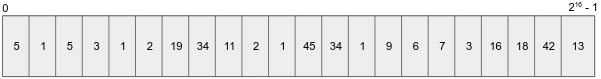
\includegraphics[width=0.7\textwidth]{rdbi-behavior-new}
    \caption{New procedure for scanning the RDBI service.}
    \label{fig:rdbi-behavior-new}
\end{figure}

This leads to one question. Which block size leads to best results? This is again answered by a simulation, which is performed for every possible block size, as such block sizes of $2^2, 2^3, ..., 2^{15}, 2^{16}$ were chosen because they are divisors for 2\textsuperscript{16}. The probability of a positive response of a block are calculated based on the results of all ECUs. The resulting coverage and speed-up are then calculated for each ECU specifically and averaged. The approach has one more feature which makes the simulation more complex than the former simulation. Since the blocks are first scanned randomly, the scan can lead to a great coverage, but also a low one, depending on the hit rate of the generated identifiers. To reduce this effect, the calculation of the coverage and speed-up are made 100 times, each time with newly created random identifiers. The 100 results are averaged to the value corrected from the random factor. This leads to a high processing time. To reduce the runtime, the execution was parallelized.
The following pseudocode shows the procedure more clearly.

\begin{samepage}
\begin{minted}{python}
for exponent in range(2, 16):
    block_size = 2 ** exponent
    coverages = []
    samples = []
    probabilities = get_probabilities(ecus, block_size)
    for ecu in ecus:
        for i in range(100):
            samples = random_samples(block_size, probabilities)
            positive_identifiers = ecu.get_positive_identifiers(samples)
            block_list = to_blocks(positive_identifiers, block_size)
            positive_identifiers = ecu.get_positive_identifiers(block_list)

            coverages.append(get_coverage(ecu, positive_identifiers))
            samples.append(len(block_list))
        avg_coverages, avg_samples = avg(coverages, samples)
\end{minted}
\end{samepage}

This simulation leads to \autoref{fig:rdbi-simulation-result}.

\begin{figure}[h]
    \centering
    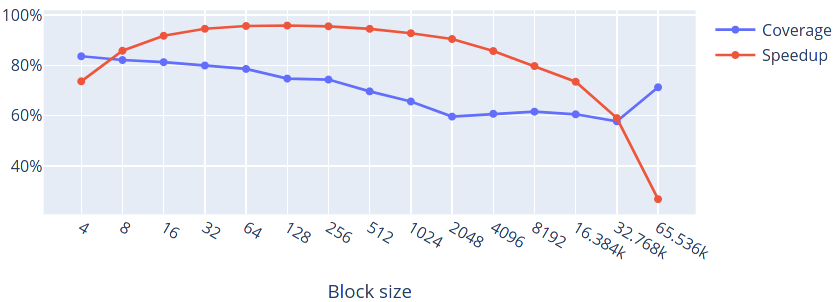
\includegraphics[width=0.8\textwidth]{rdbi-simulation-result}
    \caption{Simulation result for the RDBI service.}
    \label{fig:rdbi-simulation-result}
\end{figure}

The speed-up is no longer linear; instead, the speed-up is highest for medium block sizes. From block sizes 64 to 128, the coverage decreases by 4\% while the speed-up remains the same. Thus, it was decided for \textbf{64} as the block size leading to best results.

\subsubsection{Implementation}

Three classes are of interest again:

\begin{itemize}
    \item \textbf{RDBIEnumerator}: Defaults to scanning the whole RDBI service.
    \item \textbf{RDBIRandomEnumerator}: Scanning block-based with random identifiers.
    \item \textbf{RDBISelectiveEnumerator}: Staged enumerator containing an RDBIRandomEnumerator and an RDBIEnumerator.
\end{itemize}

\begin{figure}[h]
    \centering
    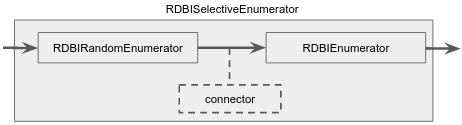
\includegraphics[width=0.7\textwidth]{rdbi-schematic}
    \caption{Schematic illustration of the new RDBISelectiveEnumerator.}
    \label{fig:rdbi-schematic}
\end{figure}

Similar to the previous approach, the new implementation is two-staged. First, the RDBIRandomEnumerator is executed. The connector creates requests for whole blocks, if any identifier of them answered positively. These requests are passed to the configurable RDBIEnumerator. Of course, it is ensured that for a single block each identifier is generated only once.

Also, as with the RCSelectiveEnumerator, each positively answered identifier will be remembered for all subsequent states. This increases the coverage because most identifiers are also available in other states, but the RandomEnumerator might not detect them for each state.

Implementing the RDBIRandomEnumerator was a challenge because it must include the probabilities of occurence of positively responded identifiers for each block. With a block size of $2^6$, there would need to be a list with $\frac{2^{16}}{2^6} = 1024$ elements. Thus, it is desirable to represent this information more compactly. A better representation is based on two facts. That the probabilities are ultimately calculated to the number of samples, and that at least one request shall be generated for each block. For the former, instead of probabilities, the number of samples for each block were pre-computed instead of being computed at runtime. This simplifies the list in the sense that integers are stored instead of float values. Second, the number of samples is not stored for all blocks, but only for blocks whose number of samples is greater than or equal to 2. And blocks for which no value is stored, the value 1 is used. This automatically solves that each block is probed with at least one packet, even if its probability is 0\%. These simplifications transformed the list of 1024 elements into a dictionary of only 109 elements.

\subsubsection{Evaluation}

\begin{table}[h]
    \begin{center}
    \begin{tabular}{ccc}
        \hline
        & \textbf{Coverage} & \textbf{Speed-up} \\
        \hline
        \textbf{audi\_cgw} & 87.8\% & 85.0\% \\
        \textbf{bfft-ecu} & 88.4\% & 96.6\% \\
        \textbf{bmw-gateway-ecu-bdc} & 100\% & 96.1\% \\
        \textbf{bmw-gateway-ecu-zgw} & 94.3\% & 95.8\% \\
        \textbf{bmw-gateway-ecu2} & 83.3\% & 96.1\% \\
        \textbf{bmw-tcu} & 72.2\% & 96.3\% \\
        \textbf{bosch-ecu} & 90.7\% & 93.3\% \\
        \textbf{dashboard} & 92.4\% & 94.4\% \\
        \textbf{mercedes-ezs} & 89.3\% & 94.7\% \\
        \textbf{seppmed} & 83.0\% & 95.9\% \\
        \textbf{tesla-airbag-ecu} & 100\% & 96.4\% \\
        \hline
    \end{tabular}
    \end{center}
    \caption{Measured coverages and speed-ups on ECUs with approach 2.}
    \label{tab:evaluation-approach2}
\end{table}

Overall, the coverages are lower with this approach as for approach 1. Only for two ECUs a coverage of 100\% is reached. It should be noted, that it varies slightly for each run because a random scan is used. The speed-ups are consistently high at approximately 95\%. Nevertheless, the speed-ups of approach 1 are higher in practice, because that approach can be applied to larger service scans, and then a speed-up of about 66\% saves more time there than a speed-up of 95\% here.

The biggest problem with reducing the scan range is the newly added random factor. The coverage can be great for one scan, but low for the next one. This would require performing multiple scans using the new implementation to ensure that most identifiers were found.


\subsection{Avoid the scan of unsupported services}

Each ECU usually supports only a subset of the services offered  by the UDS standard. This approach aims to avoid scanning them in order to save requests and therefore, time.

\subsubsection{Detecting unsupported services}

The first thing to understand is how to tell if a service is supported or not. Figure 5 of the UDS standard shows the general server response behavior. In this work, it can be found in \autoref{fig:server-response-behaviour} and the important area has been highlighted.

\begin{figure}[h]
    \centering
    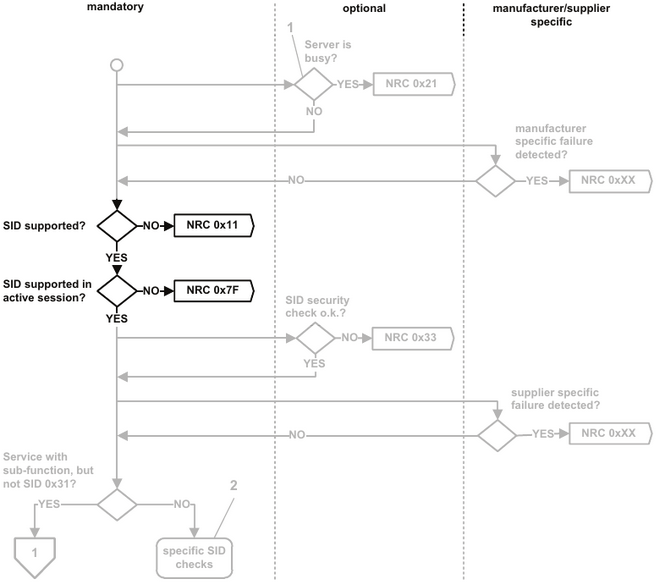
\includegraphics[width=0.8\textwidth]{server-response-behaviour}
    \caption{General server response behavior \cite{iso14229}. SID = service identifier.}
    \label{fig:server-response-behaviour}
\end{figure}

Each request is answered by a response, either positive or negative. A negative response contains a negative response code (NRC). \autoref{fig:server-response-behaviour} shows that 0x11 and 0x7f are relevant for this approach. 0x11 indicates that the requested service is not supported at all. 0x7f is a lighter response code because it shows that the requested service is not supported in the current state of the ECU. Both response codes are sufficient to stop the current enumerator with the current state and start with the next one. Although a 0x11 NRC is received, this service is still probed in other states. This is because with this behavior, in the worst case, one request is generated for this service for each state, which in turn receives 0x11 NRC again and then stops the enumerator. The number of states detected is usually one-digit, so the number of packets generated is negligible. But in the best case the vendor has implemented the NRC incorrectly and the service is available in a different state.

\subsubsection{Implementation}

In contrast to the previous approaches, this one is not applied to an enumerator, but to the UDS Scanner itself. The UDS Scanner evaluates each response, for example to detect if a new state was found. Here, a check was added for negative responses if they have the NRC 0x11 or 0x7f. If they do, the enumerator is set to completed for the currently executed state. This behavior has to be enabled explicitly, because as the next section explains, it might result in losses.

\subsubsection{Evaluation}

\autoref{fig:serviceNotSupported-savings} illustrates the number of saved packets for each ECU with this approach. It is only an approximation because for this graph, the responses with the both described NRCs have been counted. Of course, not every response can be saved with these NRCs, since at least one request must first be made to see the NRC of that service for a state. But this number of requests, as described in the previous paragraph, is very small and negligible, especially considering that the minimum value of saved requests is about 70,000.

\begin{figure}[h]
    \centering
    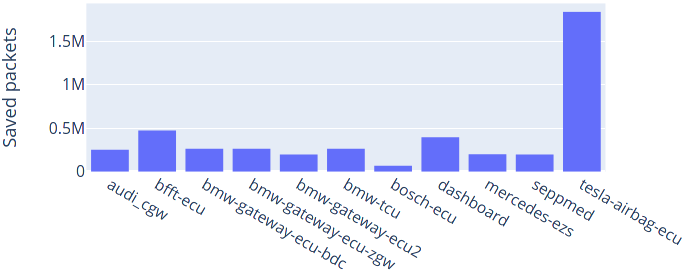
\includegraphics[width=0.8\textwidth]{serviceNotSupported-savings}
    \caption{Saved number of requests with this approach (approx).}
    \label{fig:serviceNotSupported-savings}
\end{figure}

There is one last potential problem with this approach. Reliance is placed on the manufacturer to properly implement these NRCs. It is conceivable that the ECU responds to an identifier with 0x11 or 0x7f, although a subsequent identifier would actually have been answered positively. The occurrences of this behavior are shown in \autoref{fig:serviceNotSupported-losses}. It was calculated by evaluating the responses for each enumerator for each state. Once a negative response with NRC 0x11 or 0x7f was received, an internal counter was incremented with each subsequent positive response.
And in comparison to the potential savings (\autoref{fig:serviceNotSupported-savings}), the losses are negligible.

\begin{figure}[h]
    \centering
    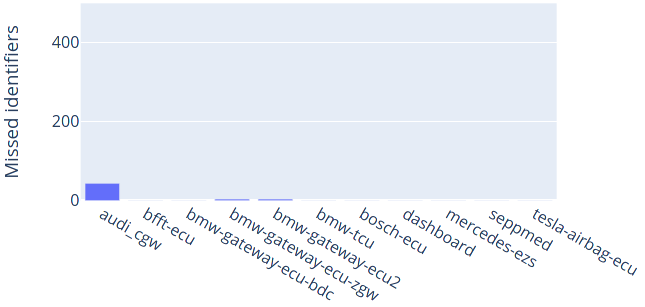
\includegraphics[width=0.8\textwidth]{serviceNotSupported-losses}
    \caption{Lost number of positive responses with this approach.}
    \label{fig:serviceNotSupported-losses}
\end{figure}

Avoiding scanning unsupported services is the safest way to save time of all three approaches. It is unlikely that identifiers will be missed, but the speed gain can still be very high.

\subsection{Actual time savings}

For each ECU, the same scans as for gathering information and profiling were executed again, they differ only in the use of the new implementations.

\begin{figure}[h]
    \centering
    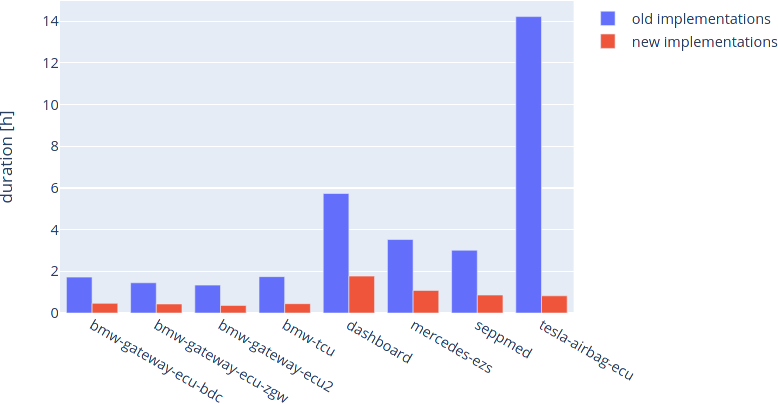
\includegraphics[width=1\textwidth]{durations-diff}
    \caption{Observed runtimes for a UDS scan with new implementations.}
    \label{fig:durations-diff}
\end{figure}

As \autoref{fig:durations-diff} illustrates, the speed-up is severe. Especially for the Tesla ECU the difference is huge.
This results from this ECU having a relatively high average response time (about 0.02 seconds) compared to the others (0.001 to 0.008 seconds).

\section{Conclusion}

\section{Conclusion and Future Work}

\subsection{Conclusion}

In this thesis, three approaches were evaluated to improve the efficiency of a UDS scan. The use of information within the same scan (approach 1), reducing the scan range (approach 2) and avoiding scanning unsupported services (approach 3).

All three approaches turned out to maintain a high speed-up while still offering a high coverage.
Nevertheless, all three approaches are not able to provide a 100\% coverage at all times. 
If a coverage of 100\% is desired, a full scan might be the preferred solution, even if it takes much longer. This may be acceptable, if this scan will be executed only once. For fast results and good, but possibly not complete coverage, the new implementation should be preferred. It depends on the use case. Therefore, the new enumerators are not a replacement for the original ones, but an addition.

\subsection{Future Work}

Reducing the scan range could also be applied to the IOCBI service. Theoretically, to many more services, but most of them only have 8-bit identifiers, leading to almost no time savings, thus not worth lower coverages.

Also, another approach can be evaluated. While elaborating this work, it was observed that manufacturers tend to use the same identifiers across their ECUs for the RDBI service. So, these identifiers could be collected, grouped by manufacturers and used for more precise scanning through fixing some requests accordingly instead of only scanning randomly. One could go one step further here and not only group by manufacturers, but also by ECU type.
For example, all available BMW ECUs turned out to have 11 identifiers in common. On the other site, the both available BMW central gateway ECUs turned out to have 61 identifiers in common. But for this approach, more data is necessary. For this work were ten unique ECUs available, which support UDS, wherein only from BMW more than one ECU was available. This is the reason why this approach was not pursued further.
For example, it turned out that all available BMW ECUs have 11 identifiers in common. On the other hand, it turned out that the two available BMW Central Gateway ECUs have 61 identifiers in common. However, more data is needed for this approach. For this work, ten unique ECUs supporting UDS were available, with only BMW having more than one available. This is the reason why this approach was not pursued.

Approach 1 and approach 2 could be merged. For example, Type1 of the RC service is no longer scanned completely, but randomly based on probabilities. Unchanged is the second stage, where Type2 and Type3 are scanned based on the results of the first stage. This probably leads to even higher speed increases, but also to lower coverages.

In addition, the UDS Scanner and enumerators are not yet part of the official Scapy repository at press time. They will be refined and gradually added to the official repository.


\include{chapters/8_closing-words}

\newpage

\ihead{References}
\nocite{*}
\printbibliography
\end{document}
